\chapter{Introduction}
We, the group 630 on the Bachelors Degree in Control, wanted to work with an unstable system for this bachelor project in control engineering. The choice fell on a form of inverted pendulum setup that is called Cubli. This structure is a cube that can jump up and balance on one of its sides or on one of its corners, as shown in \figref{CubliCorner}.
The Cubli is designed as a simple setup to let control engineers work with an inverted pendulum. A working Cubli also can be a fun thing to show the general public to explain what control engineering is about.  \cite{MGajamohan}

\begin{figure}[H] 
	\centering
	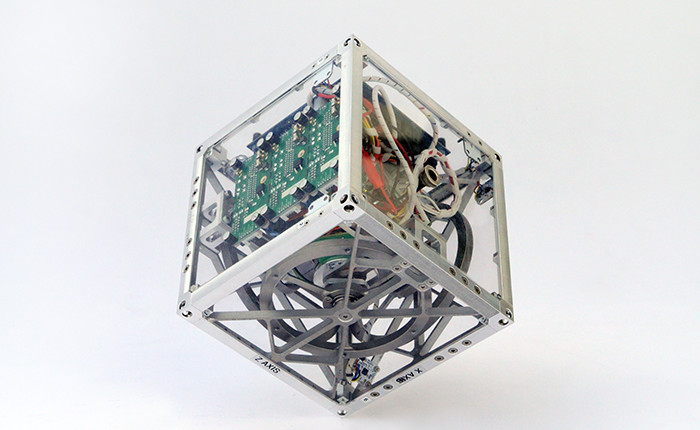
\includegraphics[scale=1.3]{figures/CubliCorner-700x430}
	\caption{A Cubli balancing on one of its corners\cite{RAndrea}}
	\label{CubliCorner}
\end{figure} 
The Cubli balances with the help of reaction wheels that spin up or down. Jumping up from a resting position is done by braking one or more of the reaction wheels, which overcomes the friction keeping the Cubli still. 
By controlling the direction of the jump-up motion and the falling direction, the Cubli can move around its body. At this point the Cubli can be considered a cube robot.\\
Applications for this cube robot, that moves without any external tools, might seem limited when you only have one cube. If you take a group of cubes, they could move together to traverse obstacles or solve puzzles one cube alone could not. A group of cubes can form a structure (\figref{MBlocksExample}), and by talking in between each other they can use their reactions wheels get the structure they are forming to move in the desired direction. Since each cube can move independently a single cube can detach for an assignment or catch up with the main structure if it gets dropped.\cite{JRomanishin}

\begin{figure}[H] 
	\centering 
	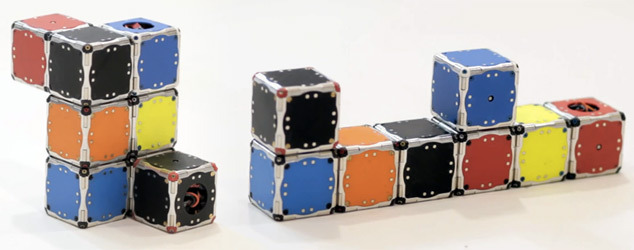
\includegraphics[scale=0.4]{figures/m-blocks}
	\caption{A number of cube robots (called M-blocks at Massachusetts Institute of Technology (MIT)) shown making two different structures. These M-blocks stick together with the help of magnets in placed in their corners\cite{LRosen}}
	\label{MBlocksExample}
\end{figure} 
At Aalborg University (AAU) there exists a working setup of a one-dimensional Cubli. The overall goal of this semester is making a model of a system, making a simulation of that and then designing and implementing a controller for that system. Students are encouraged to work with pre-made setups, since there is no extra credit for hardware solutions.



%At AAU we have a one-dimensional setup, based on the Cubli idea. It consists of a metalframe with one flywheel. In this case the inverted pendulum setup is not controlled by a motor that moves the pendulum, but by a flywheel attached to the square frame. The idea is to balance the frame on one corner with the help of the flywheel by accelerating the wheel up and down.



